\begin{figure}
% discrete_generated_nk/archive_bg16/2020-07-24 122519 9741a16
    \centering
    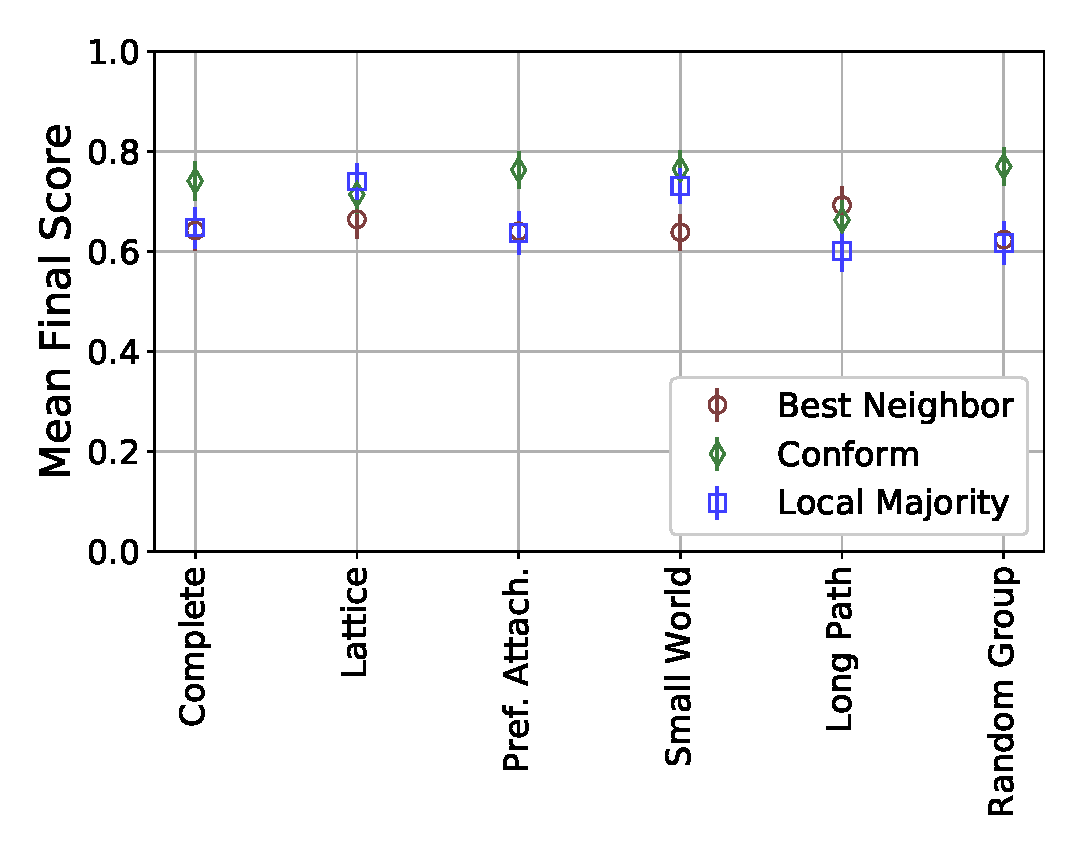
\includegraphics[width=3.25in,height=2.75in]{fig-performance-bg16.eps}
    \caption{Mean final scores for social learning on a rugged landscape with neighbor sampling (100 runs of 300 learning-step iterations). We use the same task parameters as \cite{barkoczi_social_2016} and reproduce their results: the best-neighbor strategy leads to inefficient networks (e.g., lattice) outperforming efficient ones (e.g., complete), while the conform strategy leads to efficient networks outperforming inefficient ones. We find the same result holds in the Network Deliberation setting: the best-neighbor strategy leads to the inefficient long-path group assignment outperforming random group assignment, while the conform strategy leads to the efficient random-group assignment outperforming long-path.}
    \label{fig:result-bg16}
\end{figure}

\begin{figure}
% discrete_generated_nk/archive_hybrid/2020-07-24 153547 9741a16
    \centering
    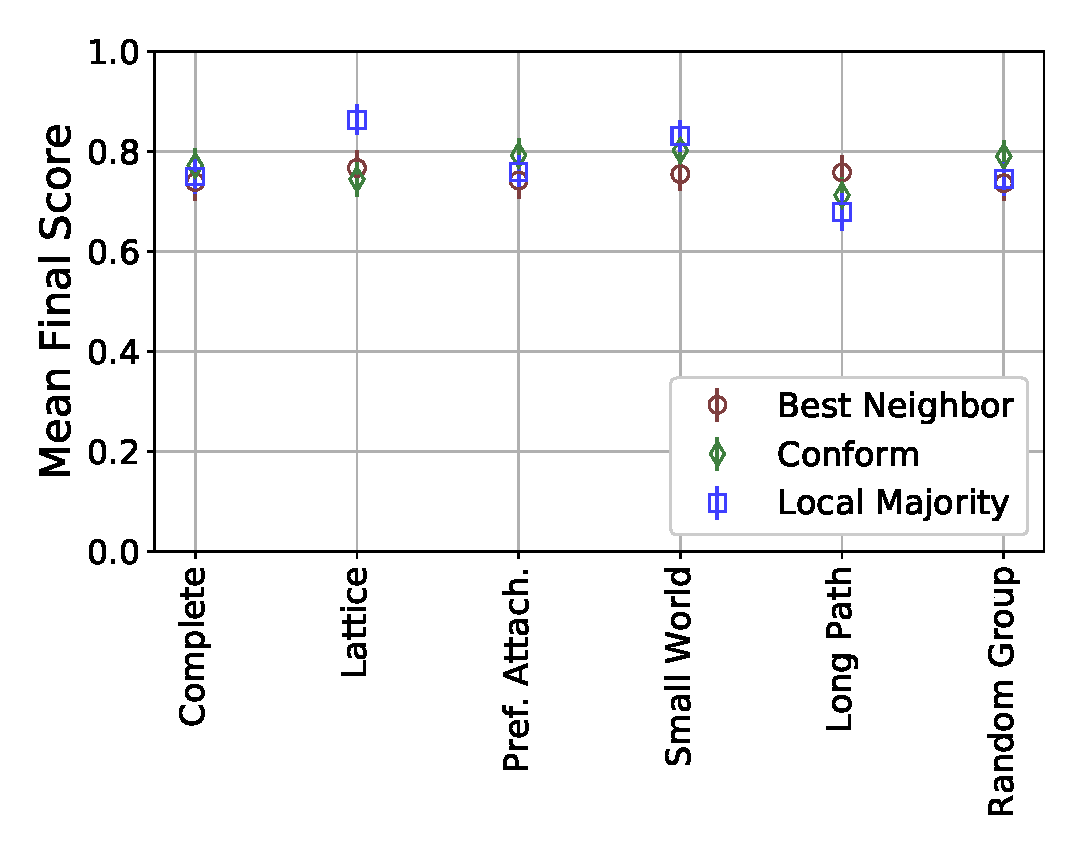
\includegraphics[width=3.25in,height=2.75in]{fig-performance-hybrid.eps}
    \caption{Mean final scores for social learning on a rugged landscape using hybrid social-indiviual learning and neighbor sampling (100 runs of 300 learning-step iterations). Performance of the conform strategy is similar to Fig. \ref{fig:result-bg16}, while the best-neighbor and local-majority strategies show improved performance across all networks.}
    \label{fig:result-hybrid}
\end{figure}

\begin{figure}
% discrete_generated_nk/archive_hybrid/2020-07-25 003254 9741a16
    \centering
    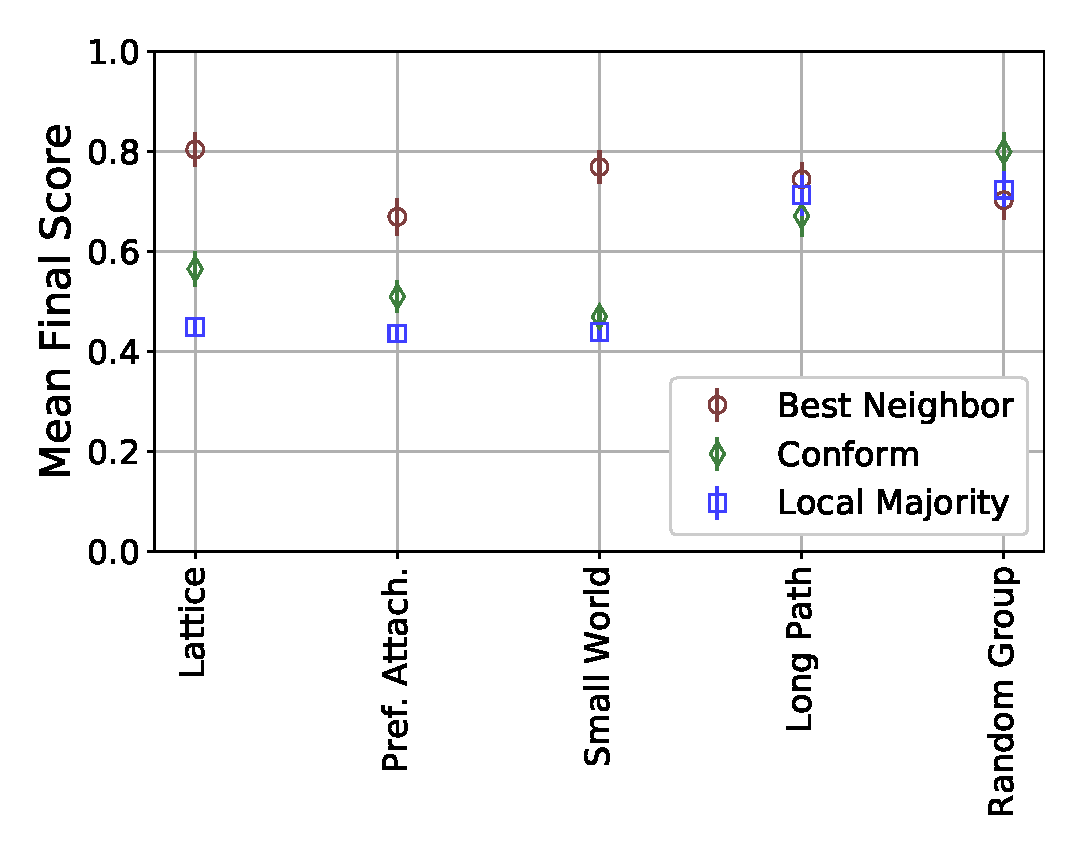
\includegraphics[width=3.25in,height=2.75in]{fig-performance-nosample.eps}
    \caption{Mean final scores for social learning on a rugged landscape using hybrid social-individual learning without neighbor sampling. Average node degree is 4. While the best-neighbor strategy shows comparable performance across all networks, the conform and local majority strategies perform significantly better in both network deliberation settings than in the single-group networks, with conform/random-group matching the best performance of any single-group setting. As with the sampling case, we find that under the best-neighbor strategy, long-path group assignment outperforms random group assignmnt, while under the conform strategy, random group assignment provides the best performance. The local-majority strategy performs similarly in both of the network deliberation settings, landing between the other two strategies.}
    \label{fig:result-nosample}
\end{figure}

\begin{figure}
% discrete_generated_nk/archive_hybrid/2020-08-14 160620 d441939
    \centering
    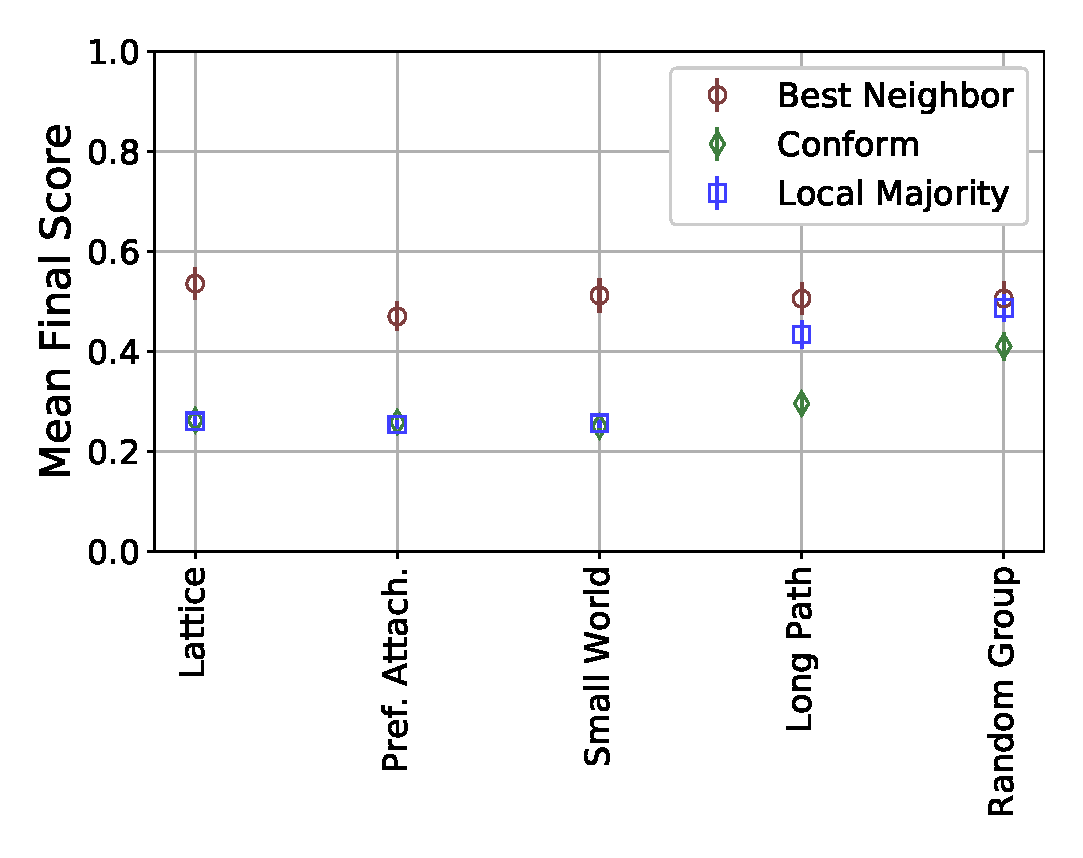
\includegraphics[width=3.25in,height=2.75in]{fig-performance-complex.eps}
    \caption{Mean final scores for social learning on a highly rugged landscape ($K=12$) using hybrid social-individual learning without neighbor sampling. Average node degree is 4. Results are similar to Fig. \ref{fig:result-nosample}, but local majority now outperforms conformity for both ND networks. Neither Best Neighbor nor Conform strategy can create a solution outside the basins of attraction already discovered, while Local Majority can. As the number of local maxima becomes much larger than the number of agents, the generative nature of the Local Majority strategy allows it to discover basins of attraction for new local maxima, increasing the probability of finding the global maximum.}
    \label{fig:result-complex}
\end{figure}

\subsection{Noisy Estimation}

\begin{figure}
% discrete_generated/archive/2020-10-07 112527 d441939
    \centering
    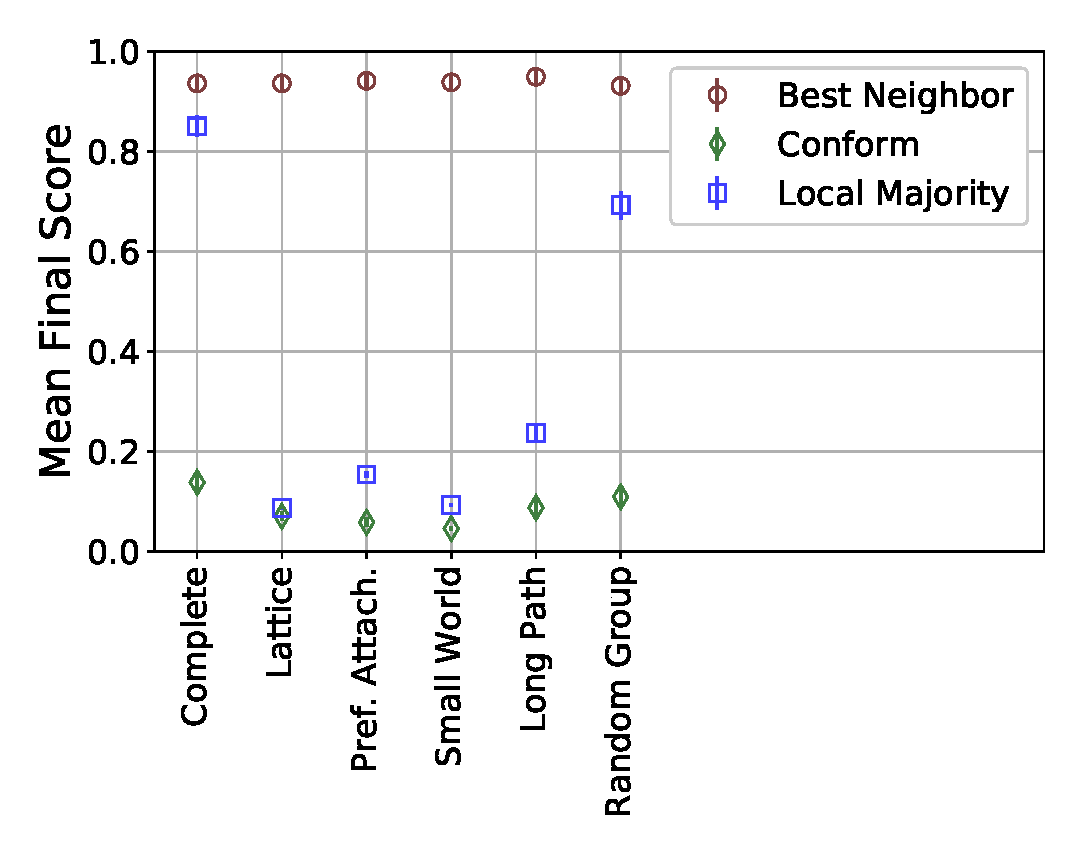
\includegraphics[width=3.25in,height=2.75in]{fig-performance-estimation-nosample.eps}
    \caption{Mean final scores for social learning on a noisy estimation task (1000 runs of 50 learning step iterations). The task consists of estimating a 7-bit target state from noisy observations. Each bit of each agent's observation has a 40\% chance of being incorrect. Average node degree is 4 (excluding complete network) and no sampling is used. The best-neighbor strategy performs well across all networks and the conform stragey performs poorly across all networks. However, the local majority strategy performs well on the complete network and for network deliberation with random group assignments.}
    \label{fig:result-nosample}
\end{figure}
